\documentclass[a4paper,11pt,UTF8]{article}
\usepackage{ctex}
\usepackage{amsmath,amsthm,amssymb,amsfonts}
\usepackage{amsmath}
\usepackage[a4paper]{geometry}
\usepackage{graphicx}
\usepackage{microtype}
\usepackage{siunitx}
\usepackage{booktabs}
\usepackage[colorlinks=false, pdfborder={0 0 0}]{hyperref}
\usepackage{cleveref}
\usepackage{esint} 
\usepackage{graphicx}
\usepackage{ragged2e}
\usepackage{pifont}
\usepackage{extarrows}
\usepackage{mathptmx}
\usepackage{float}
\usepackage{caption}
\usepackage{multirow}
\usepackage{subfigure}
\usepackage{titlesec}
\usepackage{makecell}
\usepackage{tabularx}
\usepackage{graphicx}

\titleformat{\section}{\Large\bfseries}{\thesection}{1em}{}
\titleformat{\subsection}{\large\bfseries}{\thesubsection}{1em}{}
\titleformat{\subsubsection}{\normalsize\bfseries}{\thesubsubsection}{1em}{}
\begin{document}
\title{\huge 实验报告 \\ 共源放大电路设计、仿真与实现}
\author{电子信息与通信学院 \\ 提高2301班 \\ 张禹阳 \ U202314270}

\maketitle

\begin{figure}[H]
	\centering
	\subfigure{
		
\includegraphics[scale=1]{hust.png}
	}
	\subfigure{
		
\includegraphics[scale=1]{eic.png}
	}
\end{figure}

\tableofcontents\newpage

\section{实验目的}

\begin{itemize}
    \item 集成运放性能指标含义
	\item 集成运放使用方法与注意事项
	\item 函数发生器设计方法与测试技术
	\item 两级电路的级联与调试方法
\end{itemize}

\section{实验元器件}

\begin{table}[H]
	\centering
	\begin{tabular}{|c|c|c|}
		\hline
		名称 & 型号/参数 & 数量 \\
		\hline
		运算放大器 & NE5532 & 1 \\
		\hline
		\multirow{3}{*}{电容} & 1$\mu$F & 1 \\
		\cline{2-3}
		& 0.1$\mu$F & 1 \\
        \cline{2-3}
        & 470pF & 1 \\
		\hline
		\multirow{2}{*}{电阻} & 10$\mathrm{k\Omega}$ & 2 \\
		\cline{2-3}
		& 1$\mathrm{k\Omega}$ & 3 \\
        \hline
        \multirow{2}{*}{电位器} & W104 & 1 \\
        \cline{2-3}
        & W504 & 1 \\
		\hline
	\end{tabular}
\end{table}

\section{实验任务}

已知条件:运放NE5532一只。

性能指标要求:

\begin{itemize}
	\item 频率范围:100Hz $\sim$ 1kHz,1kHz $\sim$ 10kHz;
	\item 输出电压:方波 $V_{pp} \leq$ 24V,三角波 $V_{pp}$ =6V;
	\item 波形特性:方波 $t_r<30\mathrm{\mu s}$(1kHz,最大输出时)三角波$\gamma_\Delta<2\%$
\end{itemize}

注意事项:

\begin{enumerate}
	\item 组装电路前须对所有电阻逐一测量,作好记录。 
	\item 集成运算放大器的各个管脚不要接错,尤其是正、负电源不能接反,否则极易损坏芯片。
\end{enumerate}

装调步骤:

\begin{enumerate}
	\item 由于比较器$A_1$与积分器$A_2$组成正反馈闭环电路,同时输出方波与三角波,
    故这两个单元电路需同时安装。
	\item 注意: 在安装电位器RP$_1$与RP$_2$之前,先将其调整到设计值,否则电路可能会不起振。
	\item 如果电路接线正确,则在接通电源后,$A_1$的输出$v_{o1}$为方波,$A_2$的输出$v_{o2}$
    为三角波。
	\item 在频率较低时,微调RP$_1$,使三角波输出幅度满足设计指标要求。
	\item 再调节RP$_2$,则输出频率连续可变。
	
\end{enumerate}

\section{实验原理}

下图所示的电路能自动产生方波-三角波,图中虚线右边是积分器($A_2$),
虚线左边是同相输入的迟滞电压比较器($A_1$),其中 $C_1$ 称为加速电容,
可加速比较器的翻转。电路的工作原理分析如下:

\begin{figure}[H]
	\centering
	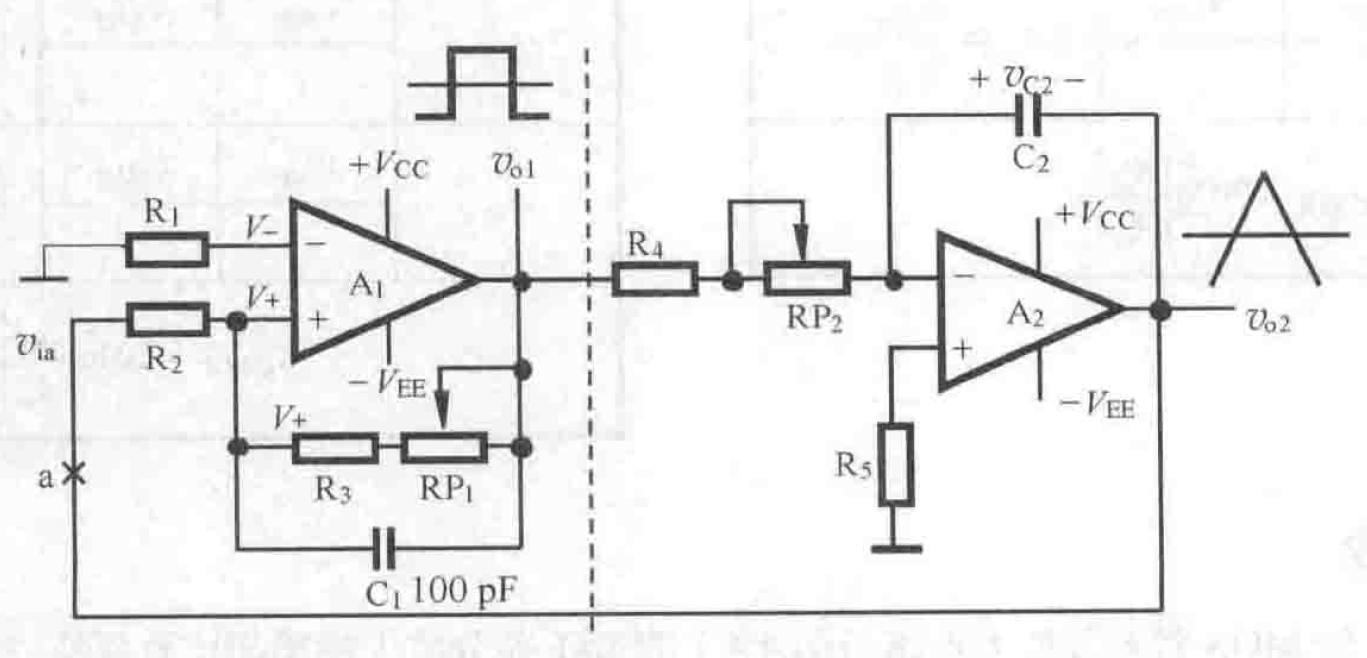
\includegraphics[width=0.7\textwidth]{3.1.png}
	\caption{原理图}
\end{figure}

若 $a$ 点断开,比较器 $A_1$ 的反相端接基准电压,即 $V_-=0$,同相端接输入电压 $v_\mathrm{ia}$; 
比较器输出 $v_\mathrm{ol}$ 的高电平 $v_\mathrm{OH}$ 接近于正电源电压+$\nu_\mathrm{cc}$,
低电平 $v_\mathrm{OL}$ 接近于负电源电压-$V_\mathrm{EE}$ (通常$|+V_{CC}|=|-V_{EE}|)$。
根据叠加原理,得到:

\begin{align}
	V_{+}=\frac{R_{2}}{R_{2}+R_{3}+\mathrm{RP}_{1}}V_{\mathrm{o1}}+
    \frac{R_{3}+\mathrm{RP}_{1}}{R_{2}+R_{3}+\mathrm{RP}_{1}}V_{\mathrm{ia}}
\end{align}

式中,RP$_1$ 指电位器的调整值(以下同)。

通常将比较器的输出电压 $v_\mathrm{ol}$ 从一个电平跳变到另一个电平时对应的输入电压称为门限电压。
将比较器翻转时对应的条件 $V_+=V_-=0$ 代入式 (4.5.1), 得到

\begin{align}
	V_{\mathrm{ia}}=\frac{-R_{2}}{R_{3}+\mathrm{RP}_{1}}V_{\mathrm{ol}}
\end{align}

设 $V_{\mathrm{ol}}=V_{\mathrm{OH}}=+V_{\mathrm{CC}}$,代入式(4.5.2)得到一个较小值,
即比较器翻转的下门限电平

\begin{align}
	V_{\mathrm{T~-}}=V_{\mathrm{ia}_{-}}=\frac{-R_{2}}{R_{3}+
    \mathrm{RP}_{1}}V_{\mathrm{OH}}=\frac{-R_{2}}{R_{3}+
    \mathrm{RP}_{1}}V_{\mathrm{CC}}
\end{align}

设 $V_{\mathrm{ol}}=V_{\mathrm{OL}}=-V_{\mathrm{EE}}=-V_{\mathrm{CC}}$,代入式(4.5.2)
得到一个较大值,即比较器翻转的上门限电平

\begin{align}
	V_{\mathrm{T}+}=V_{\mathrm{ia}+}=\frac{-R_{2}}{R_{3}+
    \mathrm{RP}_{1}}V_{\mathrm{OL}}=\frac{R_{2}}{R_{3}+
    \mathrm{RP}_{1}}V_{\mathrm{CC}}
\end{align}

比较器的门限宽度或回差电压为

\begin{align}
	\Delta V_{\mathrm{T}}=V_{\mathrm{T+}}-V_{\mathrm{T-}}=
    2\times\frac{R_{2}}{R_{3}+\mathrm{RP}_{1}}V_{\mathrm{CC}}
\end{align}

比较器的电压传输特性如图2(a)所示。当$v_\mathrm{ia}$为往复跨越上、下门限电平的电压波形时,
则 $v_\mathrm{ol}$ 不断在高、低电平之间跳变,即输出一串方波。$C_1$在 $v_\mathrm{ol}$ 
跳变瞬间可看作短路,使门限迅速改变,即运放 $A_1$的 $\nu_+$和 $\nu$之差迅速增大,
从而加速输出的翻转。$C_1$在 $\upsilon_\mathrm{ol}$ 保持高电平或低电平期间则可看作开路。

\begin{figure}[H]
	\centering
	\subfigure[比较器电压传输特性]{
		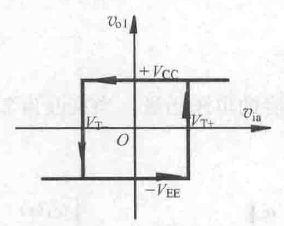
\includegraphics[width=0.3\textwidth]{3.2.png}
	}
	\subfigure[方波-三角波]{
		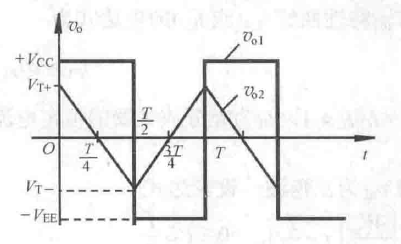
\includegraphics[width=0.4\textwidth]{3.3.png}
	}
\end{figure}

$a$ 点断开后,运放 $A_2$与 $R_4$、$RP_2$、$C_2$及 $R_5$组成反相积分器,
若积分器的输入信号 $v_\mathrm{ol}$ 为方波,则输出电压等于电容两端的电压,即

\begin{align}
	v_{02}& =-v_{\mathrm{C2}}=-\frac{1}{C_{2}}
    \int\frac{v_{\mathrm{ol}}}{(R_{4}+\mathrm{RP}_{2})}\mathrm{d}t=
    -\frac{1}{C_{2}}\int_{t_{0}}^{t_{1}}\frac{v_{\mathrm{ol}}}{(R_{4}+\mathrm{RP}_{2})}\mathrm{d}t-
    v_{\mathrm{C2}}(t_{0})\nonumber\\ &=-\frac{v_{\mathrm{ol}}}{(R_{4}+\mathrm{RP}_{2})C_{2}}(t_{1}-t_{0})+v_{02}(t_{0})
\end{align}

式中,$v_{\mathrm{C2}}(t_0)$ 是 $t_0$ 时刻电容两端的初始电压值,$v_{\mathrm{o2}}(t_0)$ 
是 $t_0$ 时刻电路的输出电压,且有 $v_{\mathrm{o2}}(t_0)=$ $-v_{C2}(t_0)$。

当$v_{01}=+V_{CC}$时,则
\begin{align}
	v_{o2}=-\frac{V_{\mathrm{CC}}}{(R_{4}+\mathrm{RP}_{2})C_{2}}\big(t_{1}-t_{0}\big)+v_{02}\big(t_{0}\big)
\end{align}

当$v_{01}=+V_{CC}$时,则
\begin{align}
	v_{02}=\frac{V_{\mathrm{CC}}}{(R_{4}+\mathrm{RP}_{2})C_{2}}\big(t_{1}-t_{0}\big)+v_{02}\big(t_{0}\big)
\end{align}

可见,当积分器的输入为方波时,输出是一个下降速率与上升速率相等的三角波,其波形关系如图2(b)所示。

$a$ 点闭合,即比较器与积分器首尾相连,形成闭环电路,只要积分器的输出电压 $\upsilon_\mathrm{o2}$ 
达到比较器的门限电平,使得比较器的输出状态发生改变,则该电路就能自动产生方波-三角波。

由图 4.5.4 所示的波形可知,输出三角波的峰-峰值就是比较器的门限宽度,即
\begin{align}
	V_{\mathrm{o2pp}}=\Delta V_{\mathrm{T}}=\frac{2R_{2}}{R_{3}+\mathrm{RP}_{1}}V_{\mathrm{CC}}
\end{align}

积分电路的输出电压 $v_\mathrm{oz}$从 $\nu_\mathrm{T}-$上升到 $\nu_\mathrm{T+}$
所需的时间是振荡周期的一半,即在 T/2 时间内 $v_\mathrm{o2}$ 的变化量等于$V_\mathrm{o2pp}$。
根据式(4.5.8)得到电路的振荡周期为
\begin{align}
	T=\frac{4R_2(R_4+\mathrm{RP}_2)C_2}{R_3+\mathrm{RP}_1}
\end{align}

方波-三角波的频率为
\begin{align}
	f=\frac{1}{4(R_4+\mathrm{RP}_2)C_2}\cdot\frac{R_3+\mathrm{RP}_1}{R_2}
\end{align}

由式(4.5.9)及式(4.5.11)可以得出以下结论: 

(1) 方波的输出幅度约等于电源电压+$\nu_\mathrm{cC}$,三角波的输出幅度
与电阻$R_2$与($R_3+{RP}_1)$ 的比值有关,且小于电源电压+$\nu_\mathrm{\epsilon C}$。
电位器 RP$_{1}$可实现三角波幅度微调,但会影响方波-三角波的频率。

(2) 电位器 RP$_{2}$ 在调整输出信号的频率时,不会影响三角波输出电压的幅度。
因此应先调整电位器 RP$_1$,使输出三角波的电压幅值达到所要求的值,然后再调整电位器 RP$_2$,
使输出频率满足要求。若要求输出频率范围较宽,可取不同的$C_{2}$来改变频率的范围,
用 RP$_{2}$实现频率微调。

\section{实验过程}

安装电路前,测量得到各电阻实际值如下:

\begin{table}[H]
    \centering
    \begin{tabular}{|c|c|c|c|c|}
        \hline
        $R_1$ & $R_2$ & $R_3$ & $R_4$ & $R_5$ \\
        \hline
        9.873 $\mathrm{k\Omega}$ & 972.2$\Omega$ & 986.1$\Omega$ 
        & 979.4$\Omega$ & 9.831$\mathrm{k\Omega}$ \\
        \hline
    \end{tabular}
\end{table}

\subsection{第一档频率范围}

选取的电容为 $C_2 = 1\mu F$,调节 RP$_1$ 至 3.014 $\mathrm{k\Omega}$不变,
再调节 RP$_2$,得到上、下限频率对应的各项指标如下表格:

\begin{table}[H]
    \centering
    \begin{tabular}{|c|c|c|c|c|}
        \hline
         & 方波频率 & 方波峰峰值 & 三角波峰峰值 & 方波上升时间 \\
        \hline
        上限 & 1.003kHz & 20.40 & 6.000 & 11.12$\mathrm{\mu s}$ \\
        \hline
        下限 & 100.4Hz & 20.80 & 6.200 & 23.12$\mathrm{\mu s}$ \\
        \hline
    \end{tabular}
\end{table}

调节 RP$_2$ 至 1.012 $\mathrm{k\Omega}$,得到的方波和三角波波形如下:

\begin{figure}
    \centering
    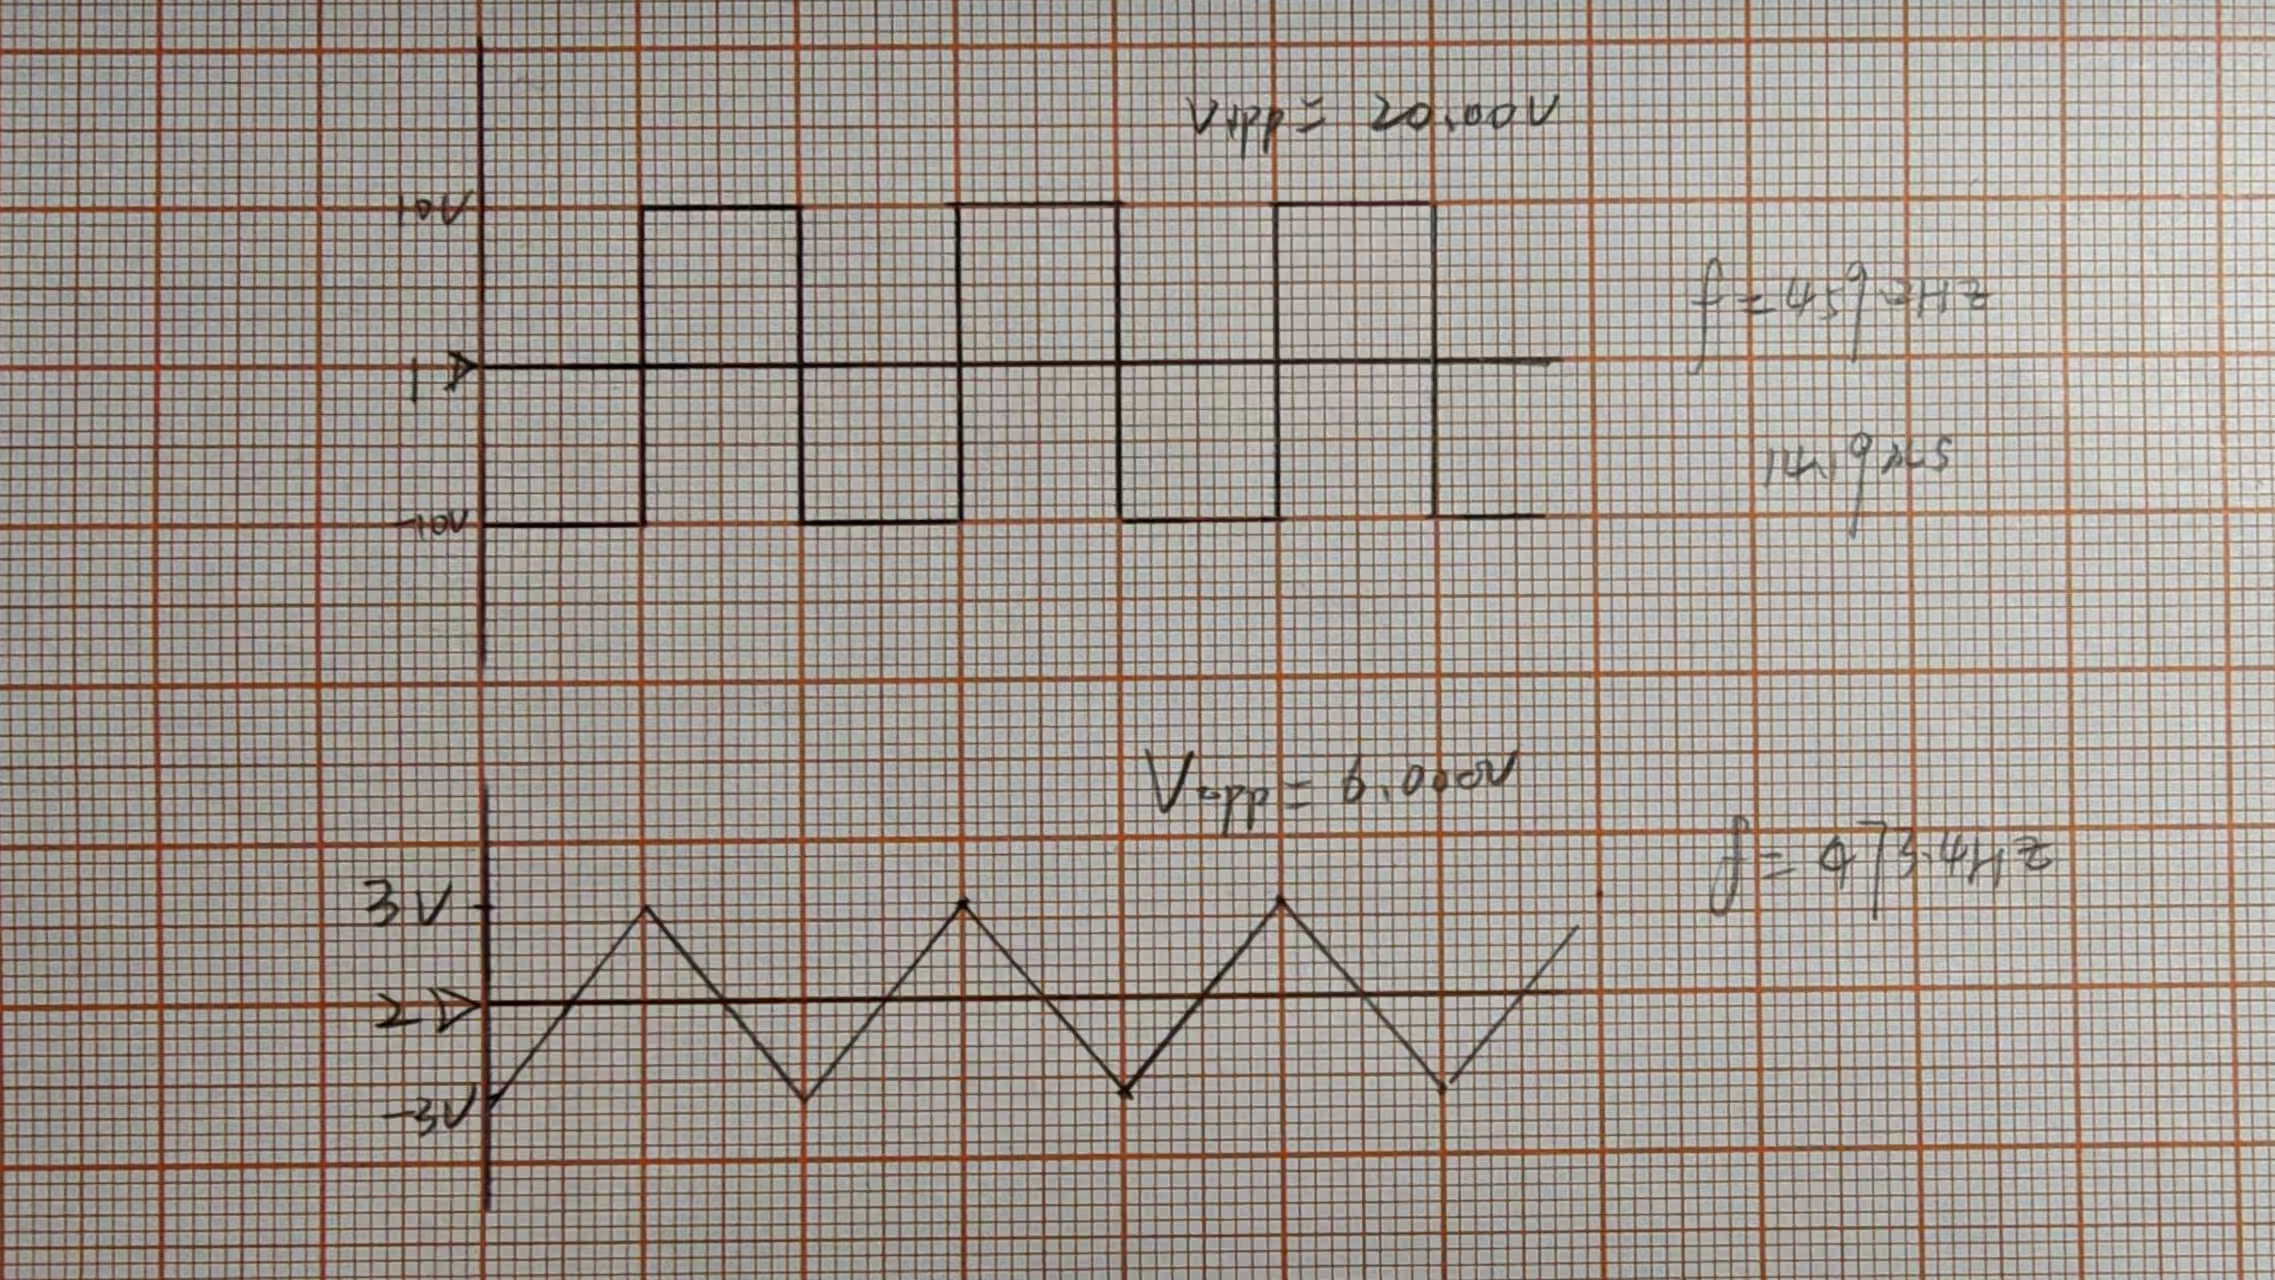
\includegraphics[width=0.7\textwidth]{3.4.jpg}
    \caption{第一档频率范围典型波形}
\end{figure}

根据实际测量得到的电阻值计算频率和三角波峰峰值的理论值,并与实际值比较,结果如下表格:

\begin{table}[H]
    \centering
    \begin{tabular}{|c|c|c|c|}
        \hline
         & 理论值 & 实际值 & 相对误差 \\
        \hline
        频率 & 516.5Hz & 459.2Hz & 11.1 \% \\
        \hline
        三角波峰峰值 & 5.833$\mathrm{V}$ & 6.000$\mathrm{V}$ & 2.86 \%\\
        \hline
    \end{tabular}
\end{table}

\subsection{第二档频率范围}

选取的电容为 $C_2 = 0.1\mu F$,调节 RP$_1$ 至 3.014 $k\Omega$不变,
再调节 RP$_2$,得到上、下限频率对应的各项指标如下表格:

\begin{table}[H]
    \centering
    \begin{tabular}{|c|c|c|c|c|}
        \hline
         & 方波频率 & 方波峰峰值 & 三角波峰峰值 & 方波上升时间 \\
        \hline
        上限 & 10.27kHz & 19.80$\mathrm{V}$ & 5.900$\mathrm{V}$ & 7.860$\mathrm{\mu s}$ \\
        \hline
        下限 & 1.013Hz & 20.00$\mathrm{V}$ & 6.000$\mathrm{V}$ & 8.204$\mathrm{\mu s}$ \\
        \hline
    \end{tabular}
\end{table}

调节 RP$_2$ 至 1.012 $k\Omega$,得到的方波和三角波波形如下:

\begin{figure}
    \centering
    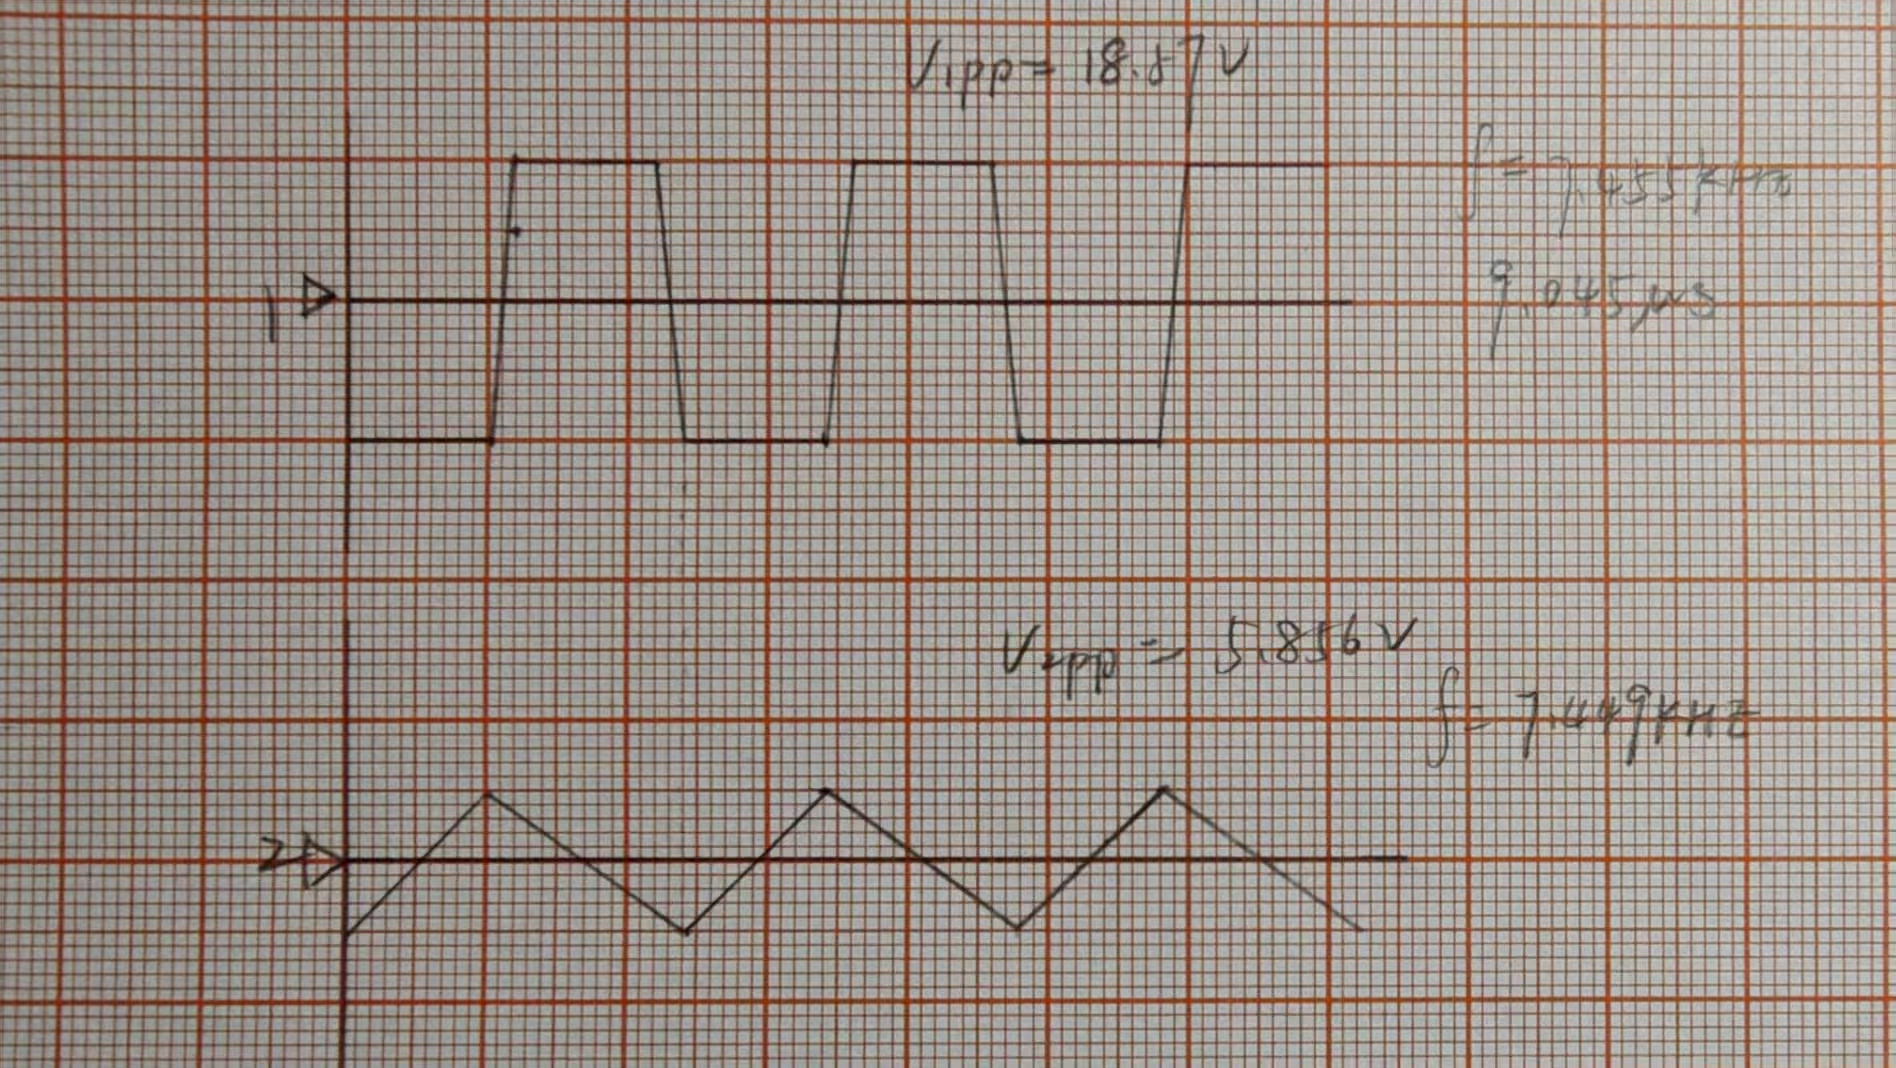
\includegraphics[width=0.7\textwidth]{3.5.jpg}
    \caption{第二档频率范围典型波形}
\end{figure}

根据实际测量得到的电阻值计算频率和三角波峰峰值的理论值,并与实际值比较,结果如下表格:

\begin{table}[H]
    \centering
    \begin{tabular}{|c|c|c|c|}
        \hline
         & 理论值 & 实际值 & 相对误差 \\
        \hline
        频率 & 5.165kHz & 7.455kHz & 44.6 \% \\
        \hline
        三角波峰峰值 & 5.833$\mathrm{V}$ & 6.000$\mathrm{V}$ & 2.86 \%\\
        \hline
    \end{tabular}
\end{table}

\section{实验小结}

本次实验电路我搭建得比较快,但一开始 RP$_2$ 选用的是 W103,导致在调节第二档频率时
无法调到1kHz及以下,后面发现 RP$_2$ 选得太小了,改用为 W504 后便可以顺利调节了。


\end{document}